\chapter{Funnels}

The term \funnel first appears in \cite{masonMechanicsManipulation1985}. The
\funnel definitions in this thesis is taken from a series of articles on
\funnel 's \cite{tobenkinInvariantFunnelsTrajectories2010} \cite{tedrakeLQRtreesFeedbackMotion2009} \cite{majumdarRobustOnlineMotion2013}
 \cite{majumdarFunnelLibrariesRealtime2017}
 \cite{ahmadiDSOSSDSOSOptimization2017}, with the main focus being on
 \cite{majumdarFunnelLibrariesRealtime2017}. Here a \funnel\ is mathematically
 defined as
 \[
  \bar{x}(0) \in \mathcal{X}_0 \Rightarrow \bar{x}(t) \in F(t), \forall t \in \sqb{0,T}
 \]
where \(\mathcal{X}_0\) is the set of initial conditions, \(\sqb{0,T}\) the time
interval, and \(F(t)\) is the set of states that the system can be in at time
\(t\). Although this thesis concerns itself with approximating the reachable set
through \textit{Lyapunov} functions. A useful analogy is imagining the funnel
created through a \textit{Monte-Carlo} simulation, where the \funnel would
be the set of all the paths traversed by the dynamical system at hand. For a
simple car model, this could look similar to:

\begin{figure}
  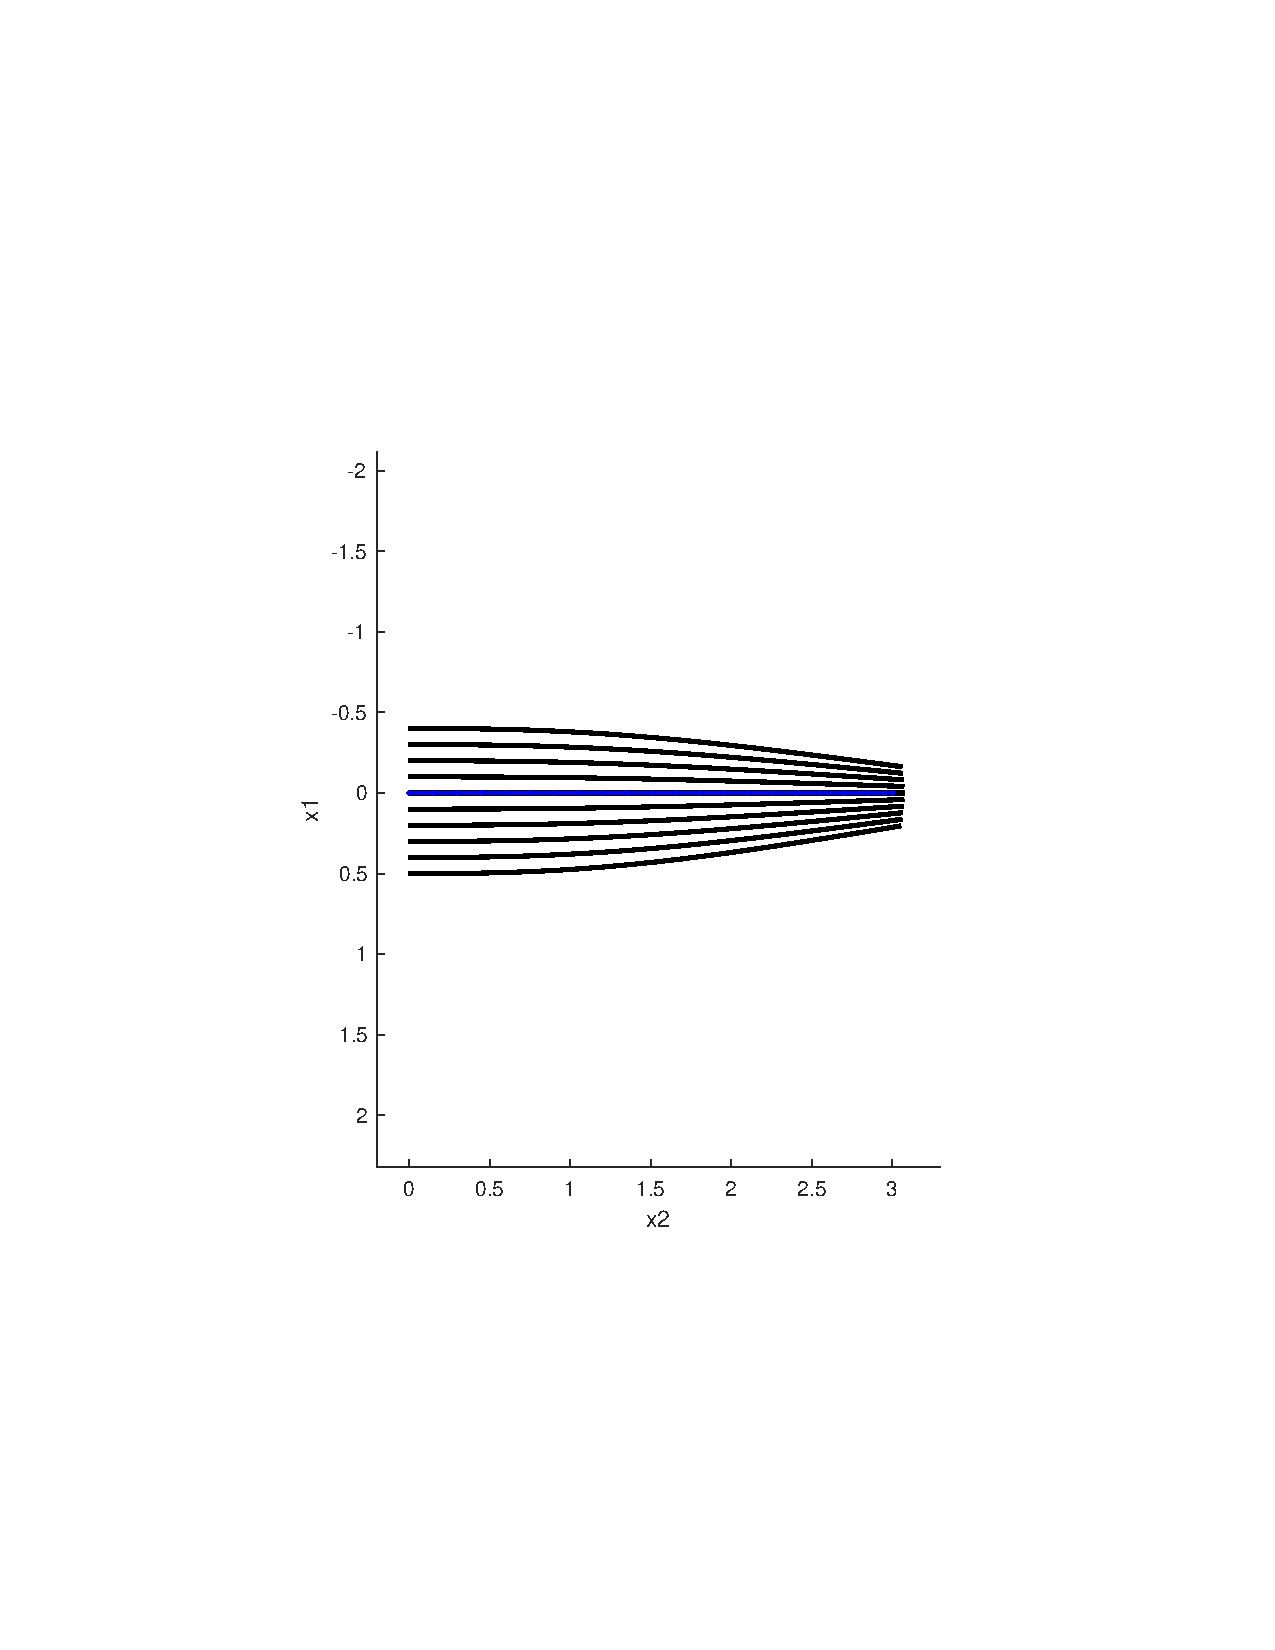
\includegraphics[scale=.5]{figures/funnels/montecarlofunnel}
  \caption{The simulation of N paths starting from a random point in the
    interval \(\sqb{-1,1}\), and controlled with a LQR controller.}
\end{figure}

\subsection{Lyapunov Functions}

A \textit{Lyapunov function} for an autonomous dynamical system is defined as a
scalar function \(V: \R^n \rightarrow \R\), with continuous first derivatives,
is locally positive definite, and \(\Delta V \dot g\) is also locally negative
definite. The \textit{Lyapunov functions} can then be used to prove the
\textit{Lyapunov stability} of the dynamical system. if \(\dot{x} = f(x)\) is a
dynamical system, and \(\dot{V}\) is the time derivate of the
\textit{Lyapunov-candidate function} \(V\), then:
\[
  \dot{V}(x) = \frac{d}{dt}V(x(t)) = \frac{\partial V}{\partial x} \cdot
  \frac{dx}{dt} = \Delta V \cdot \dot{x} = \Delta \cdot f(x)
\]

\subsection{Lyapunov Stability}

A function being stable in the sense of \textit{Lyapunov}, is defined as:
Given the autonomous nonlinear dynamical system
\[
  \dot{x} = f(x(t)), \, x(0) = x_0
\]
with \(\x(t)\) denotes the state vector of the system, with \(x(t) \in
\mathcal{D} \subseteq \R^n\). \(\mathcal{D}\) is an open set containing the
origin, and \(f \colon \mathcal{D} \rightarrow \R^n\) continous on
\(\mathcal{D}\). Suppose that \(f\) has an equilibrium at \(x_e\) so that
\(f(x_e) = 0\), then this equilibrium is \textit{Lyapunov stable} if for every
\(\epsilon > 0\) there exists a \(\delta > 0\) such that if \(\left \lVert x(0)
  - x_e \right \rVert < \delta\) then for every \(t \geq 0\) we have \( \left
  \lVert x(t) - x_e \right \rVert \leq \epsilon\).

Conceptually this means that a solution starting out in the vincinity of the
equilibrium (\(\delta\)), will remain close (\(\epsilon\)) to it. Also note that
this must be true for any \(\epsilon\) one may choose. (semicite wikipedia?).

\subsection{Lyapunov's second method for stability}

\textit{Lyapunov's} second method (also referred to as \textit{Lyapunov's} direct
method) for stability makes use of the \textit{Lyapunov} function \(V\). If
given a dynamical system of the form \(\dot{x} = f(x)\) having a point of
equilibrium at \(x = 0\). Consider a function \(V(x) \colon \R^n \rightarrow
\R\), such that
\begin{align*}
  V(x) &= 0 \text{ if and only if } x = 0 \\
  V(x) &> 0 \text{if and only if} x \neq 0 \\
  \dot{V}(x) &= \frac{d}{dt}V(x) = \sum_{i=0}^{n} \frac{\partial V}{\partial x_i} f_i(x) \leq 0 \text{ for all values of } x \neq 0. \\
\end{align*}
Then \(V(x)\) is called a \textit{Lyapunov function} candidate and the system is
stable in the sense of Lyapunov. (semicite wikipedia).

The following sections \ref{subsec:LaSalle's invariance
  principle},\ref{subsec:LaSalle's invariance principle},\ref{subsec:Lyapunov
  analysis for linear systems},  are based on the lecture notes from
\cite{tedrakeUnderactuatedRoboticsAlgorithms2019}, and are adapted slightly for
presentation in this thesis.

\subsection{LaSalle's invariance principle}
\label{subsec:LaSalle's invariance principle}

\textit{LaSalle}'s invariance principle formalizes the convergence of a
dynamical system to an invariant set, rather than to a fixed point. Defined as:
Given a system \(\dot{x} = f(x)\) with \(f\) continuous. If we produce a scalar
function \(V(x)\) with continous derivatives for which over an open subset
\(\mathcal{B} \in \R^n\) we have
\begin{align*}
  V(x) \geq 0, \; \dot{V}(x) \leq 0,
\end{align*}
and \(V(x) \rightarrow \infty\) as \(\norm{x} \rightarrow \infty\), then \(x\)
will converge to the largest \textit{invariant set} where \(\dot{V}(x) = 0\).
Where an \textit{invariant set}, \(\mathcal{G}\), of the dynamical system is a
set for which \(x(0) \in \mathcal{G} \Rightarrow \forall t > 0,\, x(t) \in
\mathcal{G}\). Meaning that once you enter the region of invariance, you never
leave; which will be important for our funnel calculations later on.

\subsection{Lyapunov analysis with convex optimization}
\label{subsec:Lyapunov analysis with convex optimization}

One of the primary limitations in Lyapunov analysis is that it is potentially
very difficult to come up with suitable \textit{Lyapunov} function candidates
for underactuated systems. Even if given a \textit{Lyapunov} function, simply
checking that the \textit{Lyapunov} conditions hold for all \(x\) can be
difficult. Imagine checking that \(\dot{V}\) is strictly negative for all \(x\),
except at the origin, if \(\dot{V}\) is some complicated nonlinear function over
a vector \(x\). However with recent advances in convex optimization
\cite{parilloStructuredSemidefinitePrograms}, there now exists the opportunity
to numerically search for these functions.

A natural approach to a numerical algorithm for verifying \textit{Lyapunov}
stability could be to evaluate \(V\) and \(\dot{V}\) at a large number of points
and check that \(V\) is positive, and that \(\dot{V}\) is negative. Which
\href{https://github.com/RobotLocomotion/drake/blob/master/systems/analysis/test/lyapunov_test.cc}{does in fact
work}.
But in reality we can do better, using optimization algorithms which rigourously
checks these conditions \textit{for all \(x\)}, without the need for dense
sampling. Which in actuality enables us to search for \textit{Lyapunov
  functions} in an infinite function space (which is what makes up the space of
all \textit{Lyapunov} functions).

\subsection{Lyapunov analysis for linear systems}
\label{subsec:Lyapunov analysis for linear systems}

\begin{theorem}
  Given a linear system of the form \(\dot{x} = Ax\) if one
  can find a \textit{Lyapunov function}
  \[
    V(x) = x^TPx, \; P = P^T \geqslant 0
  \]
  which also satisfies
  \[
    \dot{V} = x^TPAx + x^TA^TPx \leqslant 0.
  \]
  Then the origin is globally asymptotically stable.
\end{theorem} \cite{tedrakeUnderactuatedRoboticsAlgorithms2019}

For the linear case the existence of a quadratic \textit{Lyapunov} function is
a necesary and sufficient condition. Furthermore, a \textit{Lyapunov} function
can always be found by finding the positive definite solution to the matrix
Lyapunov equation
\[
  PA + A^TP = -Q
\]
for any \(Q = Q^T \geqslant 0\).

\subsection{The connection between Lyapunov analysis and convex optimization}

The first connection between Lyapunov analysis and convex optimization will be a
\ac{SDP}-program. In fact the Lyapunov conditions for a linear system can be
formulated in the form of an \ac{SDP} - which is a form of convex optimization.
For any problem formulated as an \ac{SDP} there exists an efficient - and
guaranteed optimal - solution. Only barring numerical difficulties.

\subsection{Numerical convex optimization}

\subsubsection{Linear programming}

\subsubsection{Semidefinite programming}

In essence 

\subsection{Example}
Give example of global and local and limit-cycle stability (ref tedrake notes
underactuated robotics 2018).

\subsection{Common Lyapunov functions for uncertain systems}
\subsubsection{Robust set-invariance}

A sub-level set of the Lyapunov function is, in comparison with the system
without uncertainties, not guaranteed that every sub-level set of the Lyapunov
function is not necessarily invariant. (Give example.).

\section{SOS}

\subsection{S-procedure}

The \textit{S-procedure} is used to check for positivity (SoS) over a region.

\section{Transformation of funnels}

\subsection{Cyclic coordinates?}

How de we transform the funnels to different angles and coordinates.

\subsection{Non-cyclic coordinates}

\subsection{Adding uncertainty to the funnels}

The funnels can take uncertainty into account. Adding this in accordance with
the paper by \cite{majumedar2013}. For now adding this for dimension (?).

\subsection{Scaling the funnels by the size of the vehicle simulated}

The model used in this thesis is a point model. As so, it is not ready for use
in simulations as is, whereas the vehicle used in the model has some given
length and width. Therefore the Funnel needs to be scaled to handle the given
size of the vehicle. TODO - how to do this proper? Check out the FunnelLibrary.m
file for an example on how to do this proper.

\subsection{Testing the funnels}

After we have generated our Funnels, it is time to test them through a
simulation. We start out by first simulating the Funnels with the uncertain
plant dynamics, and checks if the model ever leaves the verified parametrized
set. From this we get:

\begin{figure}
  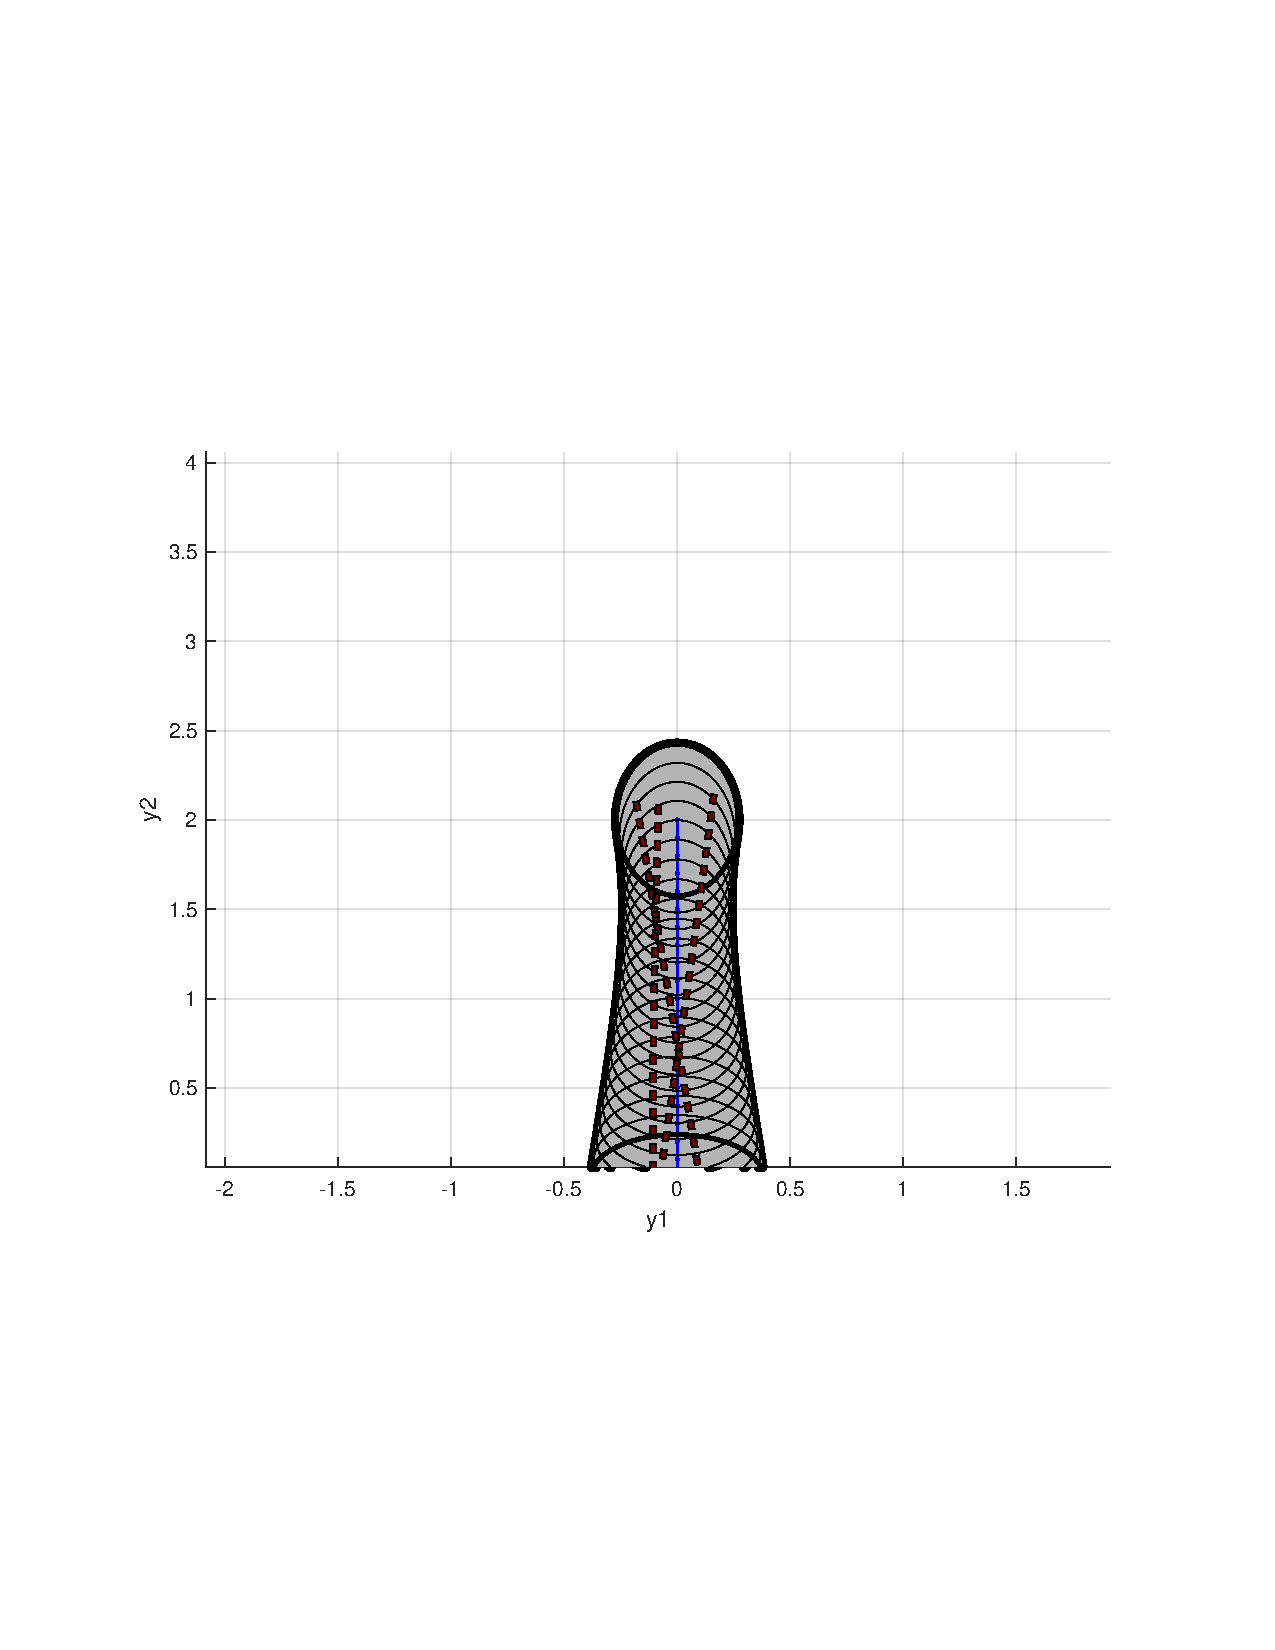
\includegraphics[scale=0.5]{figures/funnel/straight_simulation}
  \caption{Three simulations of the straight funnel with different initial
    conditions, where all three funnels stayed inside the funnel. However, they
    do seem to not converge towards the original trajectory.}
\end{figure} 


\begin{figure}
  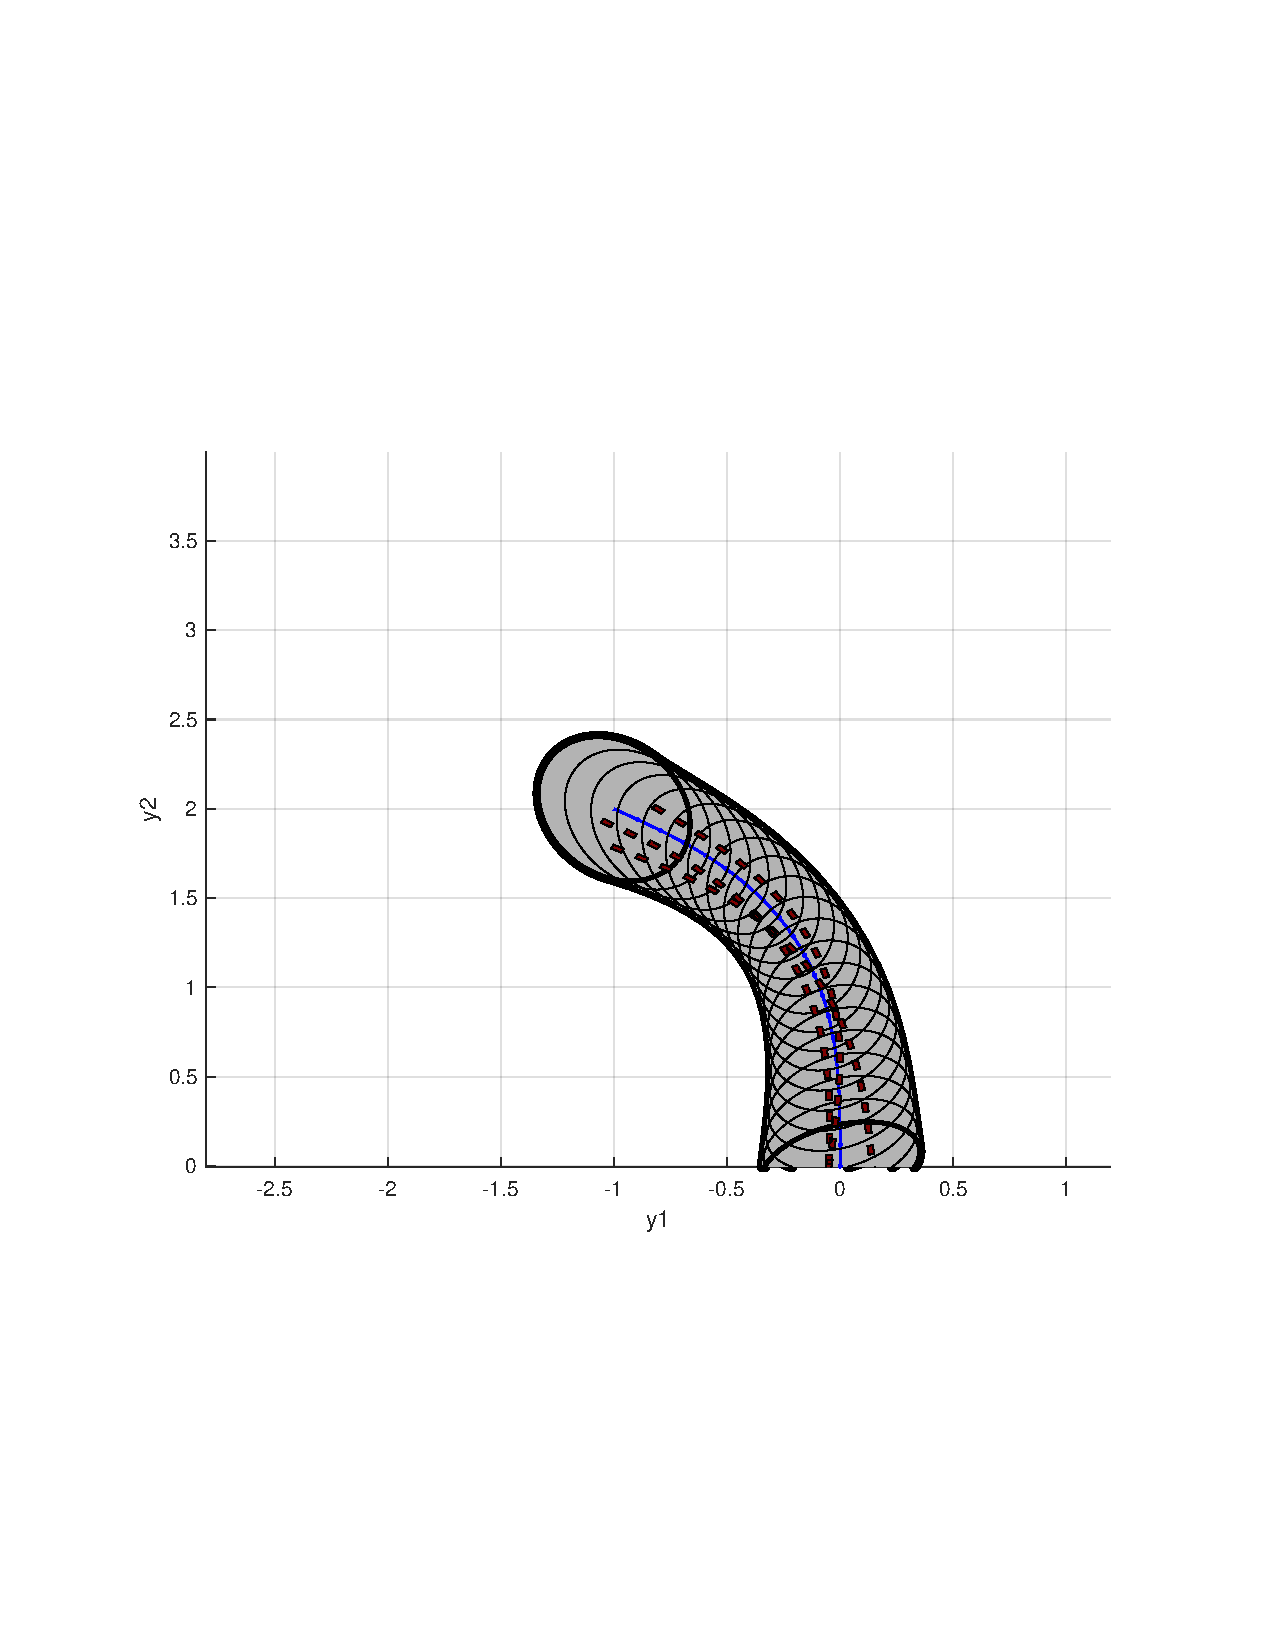
\includegraphics[scale=0.5]{figures/funnel/left_simulation}
  \caption{Three simulations of the left funnel with different initial
    conditions, where two out of three funnels left the inside of the funnel.
    Right now I can only speculate as to why this is happening.}
\end{figure} 


\begin{figure}
  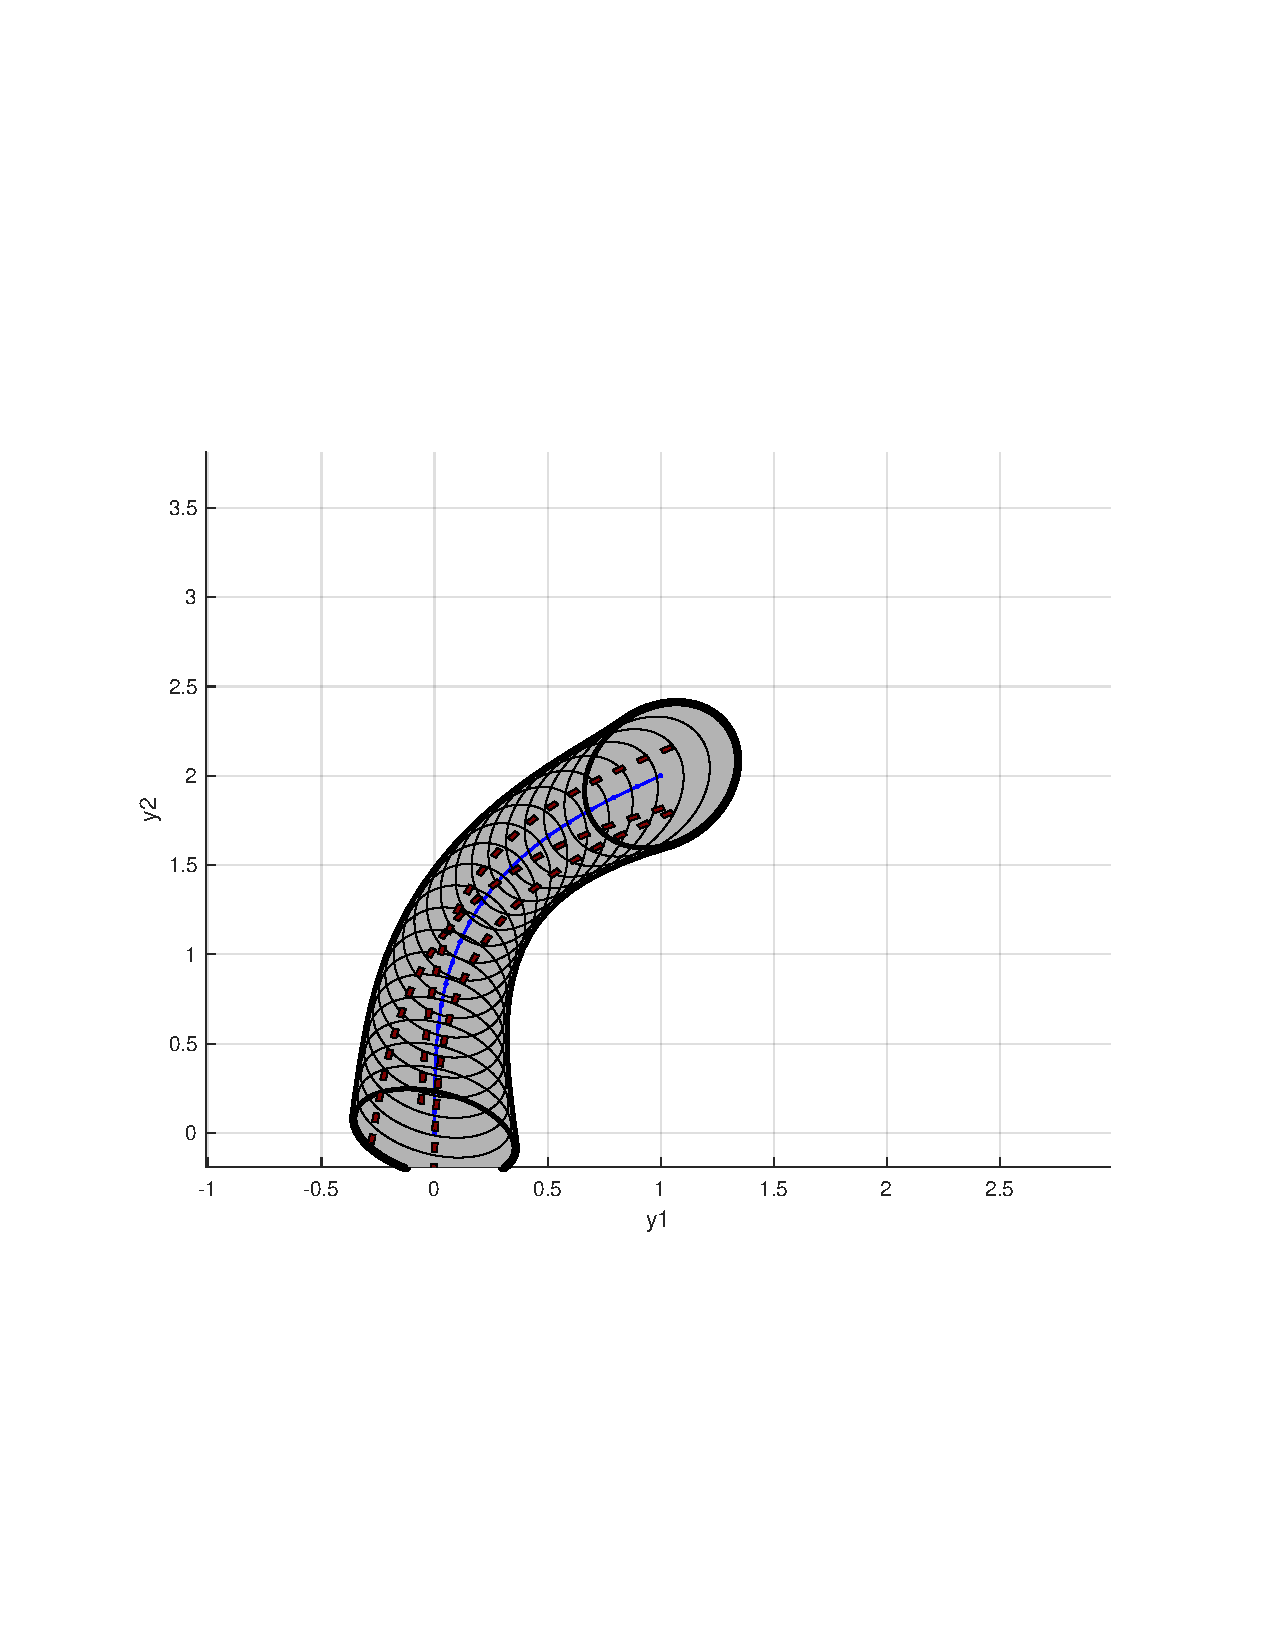
\includegraphics[scale=0.5]{figures/funnel/right_simulation}
  \caption{Three simulations of the right funnel with different initial
    conditions, where two out of three funnels left the inside of the funnel.
    Right now I can only speculate as to why this is happening.}
\end{figure} 

For the model with uncertainty added to the speed of the vehicle, we get:

\subsection{Only minimizing the volume of the funnel projected down into the xy-plane}

There is no need in minimizing the value of \(\dot{\theta}\), so in order to
minimize what we care about, i.e. the actual size of the funnel where the
physical vehicle can move, we modify our costfunction according to
\cite{majumdarFunnelLibrariesRealtime2017}. Thus, given a projection map \(\pi :
\R^n \rightarrow \R^{n_p}\). Given the ellipsoid \(\epsilon = \set{\bar{x} \in
  \R^n | \bar{x}^TS_{k}\bar{x} \leq 1}\) with
\[
  \S_k^{(p)} = (\p{PS_k^{-1}P^T}^{-1})
\]
Given that minimizing the volume of the ellipsoid \(\epsilon\) using an SDP
relies on maximizing the determinant of \(S_k\). Since \(det(S_k)\) is a
nonlinear function of \(S_k\), the function has to be linearized in order for it
to be handled by our solution framework (SOS-programming).
\cite{majumdarFunnelLibrariesRealtime2017} solves this by linearizing
\(det(S_k)\) at the solution of \(S_k\) from the previous iteration, and
maximizes this linearization instead. In the end this translates to
\[
  lin\p{det\p{S_k}} = Tr\p{P^T\p{PS_{k,0}^{-1}P^T}^{-1}PS_{k,0}^{-1}S_kS_{k,0}^{-1}}
\]
where \(S_{k,0}\) is the nominal value.
